\section{Optical properties of the sphere }
\label{sec:opt}

The central component of the experiment is the HPFS shell, which holds the LXe target, located in the center of the detector system. The shell is made of two Corning HPFS 8655 hemispheres attached by a UV transparent glue. The refractive index of HPFS 8655 is 1.575 at 185 nm (LXe R.I. 1.61); hence, there is minimal diffraction from the original direction of the photons when they 
transit from the LXe target to the sphere. The refractive indexes at various wavelengths are shown in Fig.~\ref{fig:hpfsRIcalibration} (left panel).


The HPFS transparency to VUV photons is an extremely crucial parameter for optimizing the shell's dimension. Therefore, the transmittance of an HPFS sample was measured, using a VUV monochromator light source. 
The measured transmittances as a function of wavelength are shown in Fig.~\ref{fig:hpfsRIcalibration}~(right panel). The \sout{intrinsic} transmittance of the sample at 178~\,nm, is$\sim98.7$\,\%/cm.  

\begin{figure}[h]
   \centering
   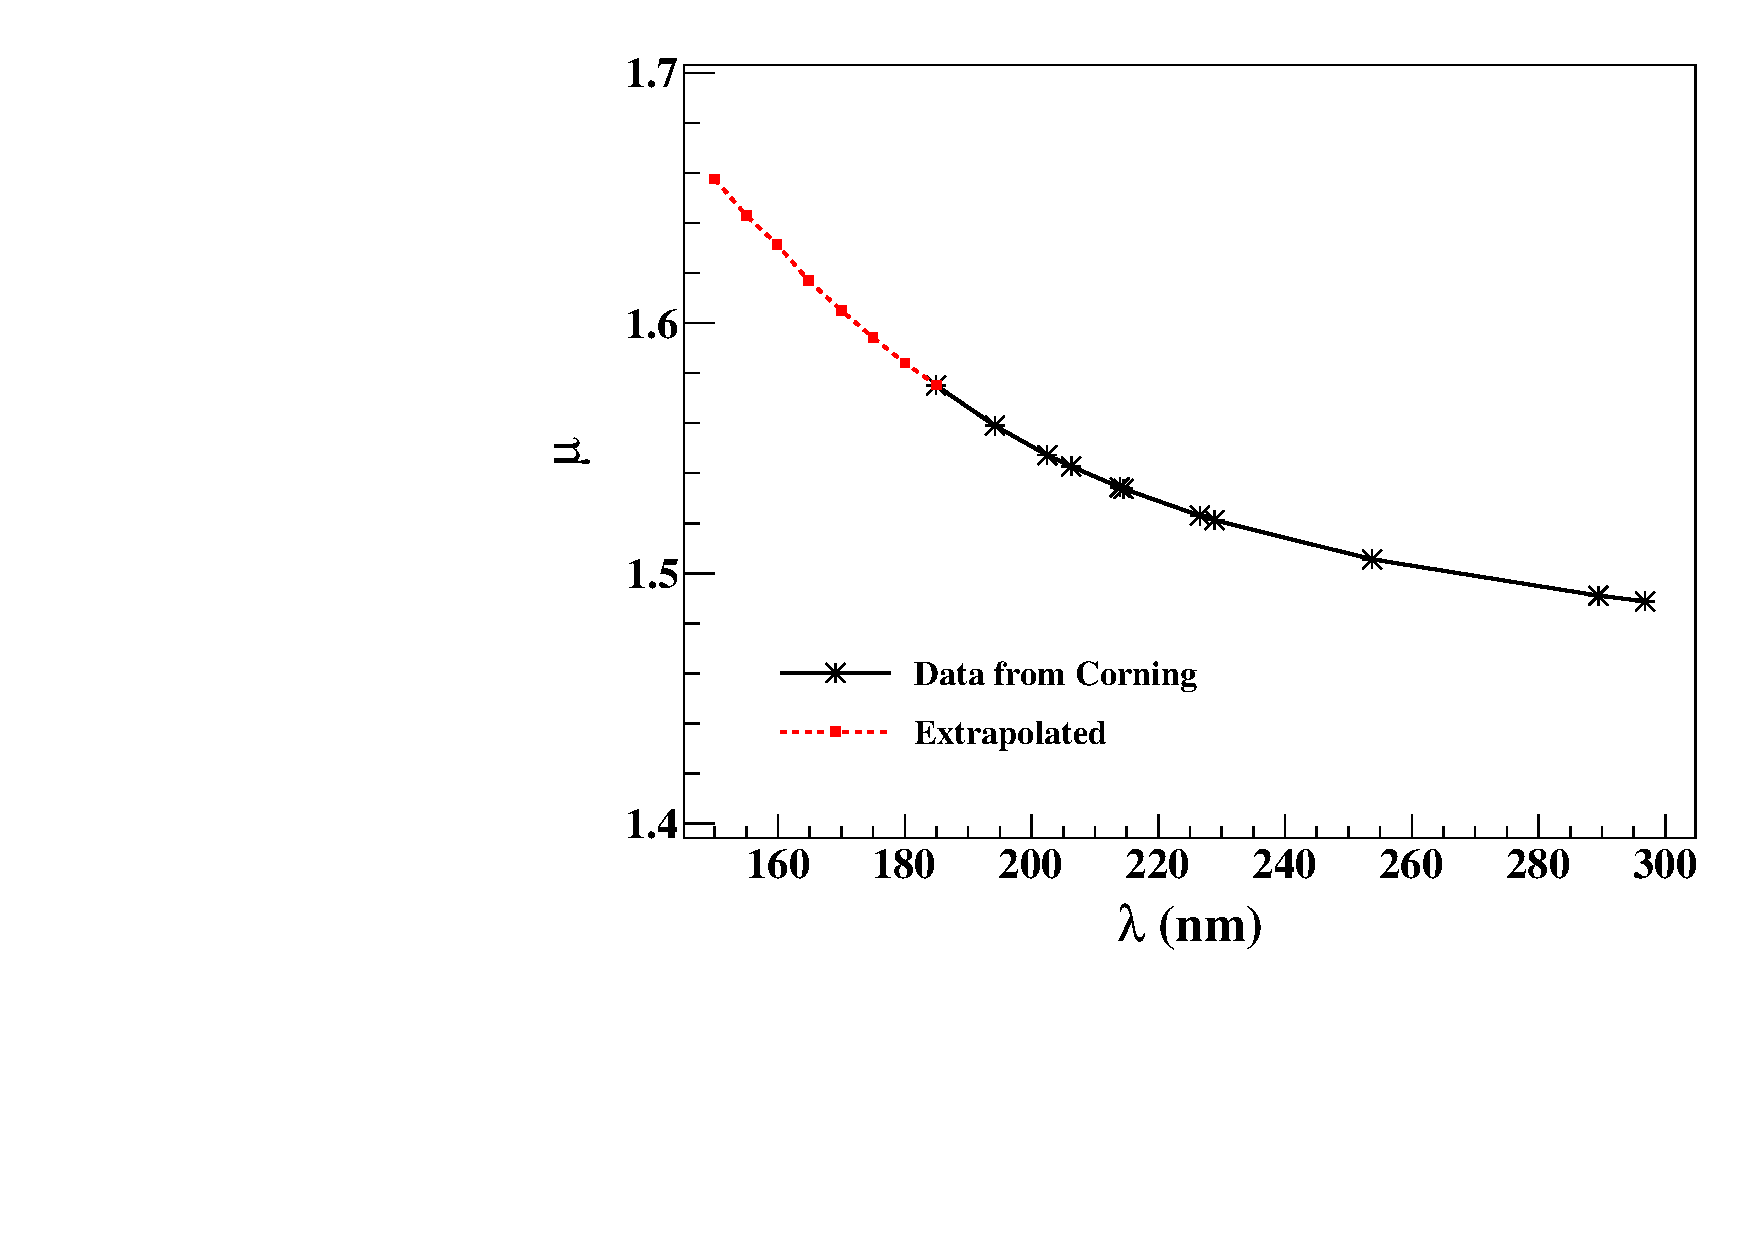
\includegraphics[width=0.48\textwidth]{RI-calibration.pdf}
    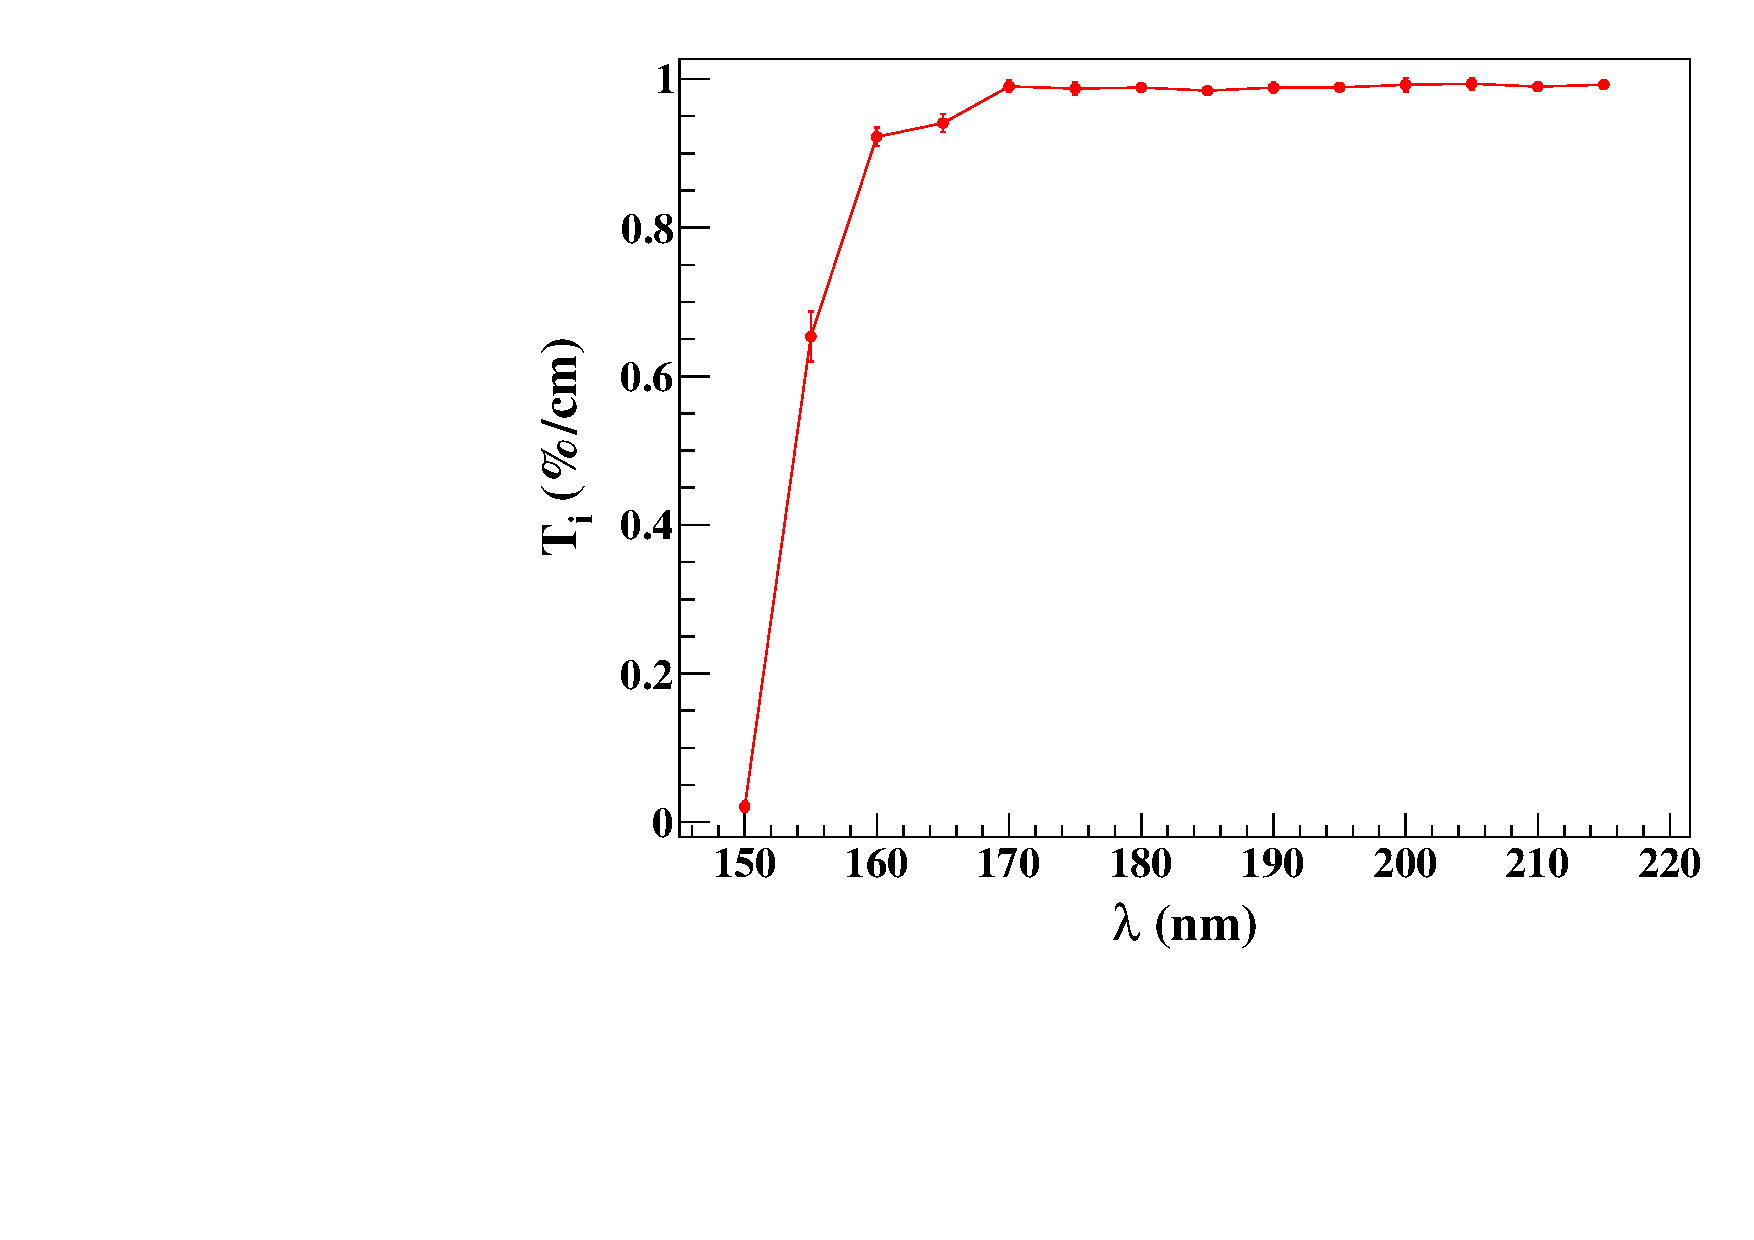
\includegraphics[width=0.48\textwidth]{IntTransmittance.pdf}
   \caption{The important characteristics of HPFS-8655. (Left) The refractive index as provided by corning and 
   extrapolated to relevant wavelength range. (Right) The internal transmittance ($T_{i}$).} 
   \label{fig:hpfsRIcalibration}
\end{figure}


The shell should be thick enough to reduce internal reflections, but not 
too thick to attenuate the scintillation light and the LXe target bubble within it should not be too large in order to avoid double scatters. The sources that will be used for exciting the xenon, and creating the supperradiance 
(signal) as well as the standard emission (background), will be $^{137} \mathrm{Cs}$ 
(662 keV) and $^{57} \mathrm{Co}$(122keV \& 136 keV) for ER and $^{241}$AmBe , 
D-D neutron generator, or neutron produced in an accelerator for NR . The mean 
free path of $^{57} \mathrm{Co}$ is a couple of mm, and for $^{137} \mathrm{Cs}$ is a couple of cm.

Using a GEANT4 based simulation~\cite{AGOSTINELLI2003250} studying the path of the scintillation photons the sphere dimensions are optimized. The outer radius (the thickness of the HPFS) is 3 cm, while the inner (the hollow space that holds the LXe) is 1 cm. 
